\section{CV basics}
\subsection*{Pinhole model}
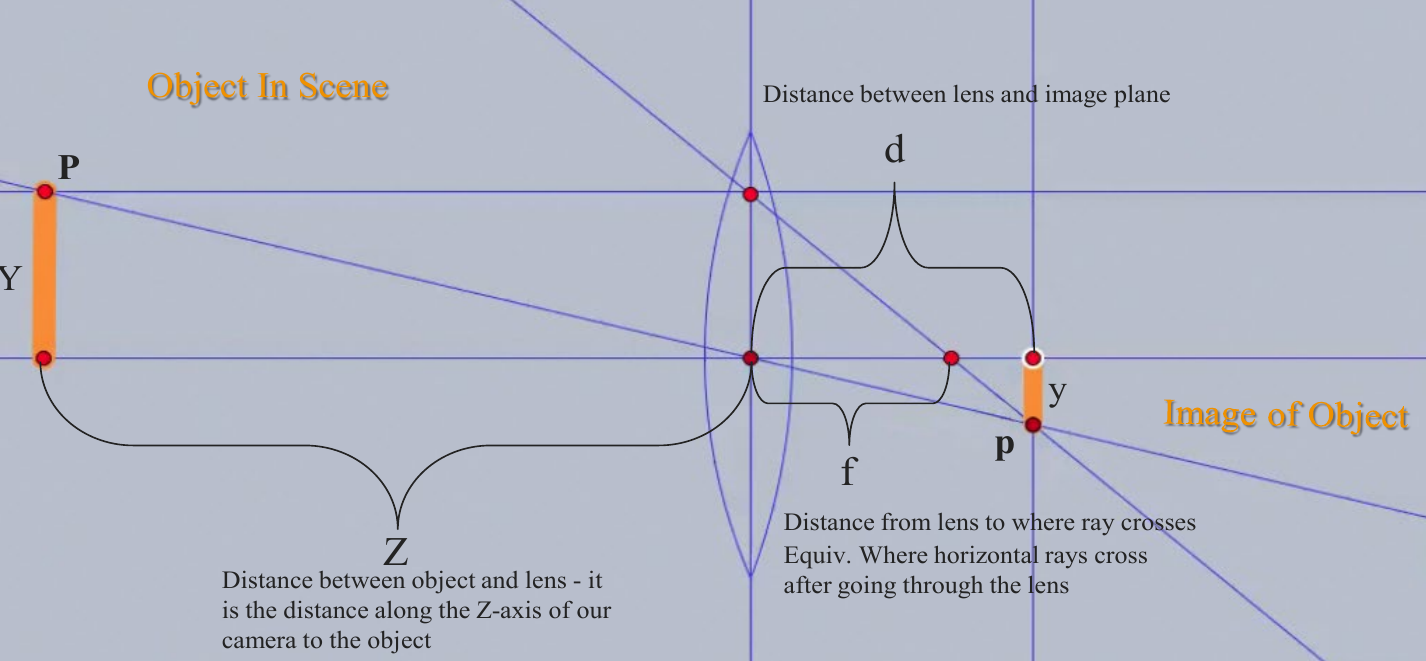
\includegraphics[width=\linewidth]{Images/Pinhole.png}
$1/f = 1/Z + 1/d$ \\
$Y/Z = y/d \Rightarrow y = d Y/Z$\\
Problem: d changes depending where the object is in the scene. Hence:
$y \approx f Y/Z$\\
\alert{Only valid if $Z >> d$}

\subsection*{Calibration Procedure}
Finds $f$ and Radial distortion:\\
$r = norm(x, y), x' = x( 1 + k_1 t + k_2 r^2
+ k_3 r^3$ (and similar for y)

\subsection*{Projection Equation}
$\begin{pmatrix} u\\ v\\ w\end{pmatrix} \sim
S \underbrace{\begin{pmatrix}r_1 & r_2 & r_3 & t \end{pmatrix}}_{^C R_W
| ^C T_W}
\begin{pmatrix} X_w \\ Y_w \\ Z_w \\ 1\end{pmatrix}$ \\
where $S = [f\,0\,x_0;\,0\,f\,y_0;\,0\,0\,1]$
\includegraphics[width=\linewidth]{Images/projection.png}

\alert{$t$ is the distance from the camera to the world coordinate
system in camera coordinates}

\subsection*{Projective Geometry}
\begin{itemize}
  \item Points at the infinity (do not intesect the 2D plane): $\begin{pmatrix} x & y & 0
    \end{pmatrix}^T$
    \item Points in the image (intersect the 2D plane): $\begin{pmatrix} x & y & 1
    \end{pmatrix}^T$
\end{itemize}

\textbf{Lines}
$\rightarrow$ represented by normal vectors 
$l^T p = 0$

\begin{itemize}
 \item Line that goes trough two points:
$l \sim p \times q$
\item intersection of two lines:
$p \sim l \times l'$
\item
if three points are collinear:
$p^T (q \times r) = 0$
\item if three lines are concurrent:
$l^T (l' \times l'') = 0$
\end{itemize}

\begin{itemize}
  \item Lines \textbf{in the image} are represented by \textbf{points in
    the infinity}
  \item Points \textbf{in the image} represent \textbf{lines in the
    infinity}.
\end{itemize}
